\section{Product Vision}
We are tasked with designing and implementing a system that allows users to upload AI scripts that can control virtual vehicles which race one another. The scripts can then be ranked according to their success. The races should be simulated on a racetrack in a virtual 3D world allowing the user to watch the race in real time. This simulation and visualization should be done using the Unity physics engine.

The product should be a complete system that can be easily used in an environment such as a careers fair. It should provide an engaging means to get students involved in some basic programming at the G-Research stand, as well as provide a starting point for further discussions and collection of contact information. However, the product should also provide systems that are deep enough for use in larger coding challenge scenarios. For example, an event where participants have a period of 2-3 hours to create the best AI script they can.  

\section{Initial Product Backlog}
After deciding on our product vision, our next step was to translate this into concrete product requirements. We decided to split these requirements into two categories: requirements that are core part of our product functioning correctly, i.e make up our Minimum Viable Product (MVP), and those that will greatly add to the product but that are not core to its functionality.
\subsection{MVP Requirements}
\begin{itemize}
\item Basic API that provides functions for controlling a vehicle:
\item Should provide information on the state of the vehicle/environment so that an AI can be created.
\item Should be simple enough for a new user to create a working script in 5/10mins.
\item Place where a user can upload a script.
\item Car physics model that can simulate and visualise a vehicle using Unity. 
\item This model should be flexible enough to allow for multiple vehicles to run simultaneously and interact.
\item Virtual racetrack that works with our car model.
\item Races should be run and displayed to the users when multiple scripts have been uploaded.
\item After a race has completed, the results should be displayed to the users and recorded.
\end{itemize}

\subsection{Stretch Requirements}
\begin{itemize}
\item Multiple racetracks.
\item Multiple vehicle types.
\item The ability to update and improve an existing script.
\item Test a script against a practice AI before submitting for a race.
\item The API should be powerful and expressive enough to write complex AI.
\end{itemize}

\section{Sprint Organisation}
We will adopt an agile way of working similar to the Scrum iterative and incremental process (see chart below). Excluding Sprint Zero, we will have two week Sprints, starting on Mondays and ending on Fridays. Our Product Owner will be Ed Cresswell from G-Research. We will not have a Scrum Master and we will use Trello instead of a physical task board.

\begin{center}
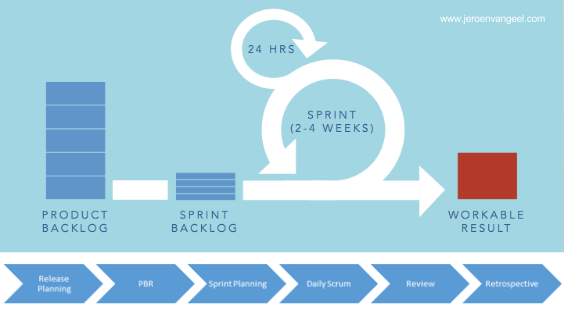
\includegraphics[scale=0.7]{sprint.png}
\end{center}

Following our initial backlog planning session, we will be meeting our Product Owner every two weeks (where possible) for Sprint reviews followed by Sprint planning - our Product Owner anticipates 3-4 meetings. If this isn�t sufficient planning time, we may arrange further planning meetings at the start of each Sprint with our supervisor. We will meet on a daily basis, but won't have a formal stand-up. 

\section{Risks and Issues}
\subsection{Organisational}
Organisational risks to be managed throughout the project:
\begin{itemize}
\item We will not have frequent meetings with our Product Owner, which may make it difficult for them to communicate their requirements and consequently steer our development.
\item It is inevitable we will overestimate or underestimate our ability to deliver on the stories we have committed to in a given Sprint -  we aren�t experienced working in a formalised agile way.
\item It may be difficult to expose every group member to all the new technologies we are using. This will make it harder for us to fill in for one another flexibly when some team members aren�t available.
\item All team members will have a variety of commitments that conflict with this project�s organisation and reduce their availability, e.g. interviews for jobs/placements.
\end{itemize}

\subsection{Ongoing}
Ongoing issues which we must consider and resolve where possible:
\begin{itemize}
\item We are producing a product on behalf of G-Research, so there are questions relating to the final product shipping:
\begin{itemize}
\item G-Research will be pitching this same project to both Cambridge and Oxford.
\item G-Research will want ownership of the project.
\item We will be developing a self-contained project that isn�t tied to G-Research�s software frameworks.
\end{itemize}
\item We must ensure that the frameworks, libraries and resources we are using have suitable licenses, considering that we are developing the product for use in a corporate environment.
\end{itemize}

\section{Estimation of Work}
Sprint Zero was an opportunity to gauge the rate at which we worked as a group, to assist in future estimation. We swiftly developed an entire slice of our software stack - we created a basic prototype to give us an idea of the difficulty of our planned features. For example, within a few days we created a car model in Unity that met our simulation requirements. Off the back of this we�ve increased our product scope to include more elaborate car physics and expect to spend a lot of time on stretch requirements (e.g. multiple vehicle types and introducing powerups). This also influenced our thinking when estimating the size of future tasks. We now expect that physics work in Unity will take less time than we initially estimated.

We are using story points as a metric to measure the amount of effort required to implement a story. These points are displayed on each Trello to easily differentiate major and minor tasks. As the project progresses, we will compare the total story point difference between tasks planned and tasks completed in each Sprint. This should indicate whether we under or overestimate workload during Sprint Planning. As we have worked in numerous group projects together, we already have a rough baseline in our minds for estimating task size. We have used this notion when assigning story points to tasks in our backlog.

\section{Creating a Plan}
The first day of our project began with a struggle - a serious lack of direction. We were given a short paragraph describing our task, and unfortunately that was all the instruction we had for two weeks of work. While most groups met with their supervisors within the first few days, our product owner was hard to reach as we couldn�t contact him directly (Our group $\rightarrow$ Marc, Imperial contact $\rightarrow$ Emily, G-Research HR $\rightarrow$ Ed, G-Research product owner). Due to the difficulty in communicating with our product owner, we were unable to setup an initial planning meeting until close to our first deadline.  In fact, for our first week we were unsure if the meeting would occur at all.

So we were faced with a hard decision, should we hold off on development until we could form a plan with Ed, or carry on undirected? It was clear that both options had risks, if we coded our own vision it could be rejected by our client and result in a huge waste of our time. And yet, if we were to stall for that initial meeting we might have to keep pushing back our work until it was deadline night, whereby our work would be reviewed the next morning!
Ultimately we chose to charge on unaided, believing some progress is better than none, which strongly influenced the evolution of our plan. 

A key component to the success of a group lies within it�s ability to stay self motivated. With the looming threat of our work being scrapped when our first meeting arrived, we delegated work by interest. Ensuring that everyone was coding parts they were excited to be coding allowed us to justify working hard even if the project went in the wrong direction and had to be scaled back.

Clients are well known for their sudden changes in requirements and wishes (and we hadn�t even met this client yet) so our plan had to be flexible enough to handle just about anything. To maintain this flexibility we frequently discussed our progress, trying to place ourselves in G-Research�s shoes and imagining what they would want us to achieve. Wherever possible we focused on work that had to be done regardless of a change in requirements. Tasks such as setting up the VM, installing development tools, and learning about technologies directly specified in the project description - such as Unity.

We began Sprint Zero with a short sighted approach to planning, focusing on what we could achieve today rather than working toward a long time goal. While this made sense before meeting our PO Ed, afterwards we had more of G-Research�s goals in mind, specifically that we were designing our project to be used at a career fair. With this new insight we refocused our direction and aimed to simplify our API. This was one of the few changes we had to make after meeting Ed, highlighting how successful we were in producing code unlikely to change in the face of changing requirements. Despite having now met Ed and having hashed out various requirements and desires, we will constantly update our plan as we tick off requirements and have further discussions with Ed.
\section{Tracking Progress and Managing Work}
To track our progress on this project we are maintaining a Product Backlog and Sprint Backlog. Our Product Backlog lists all of the features that the client requires in the final product, as well as some possible extensions. The Sprint Backlog tracks items that are to be completed within the current two week Sprint, and are filled from the Product Backlog. The features with the highest priority in the Product Backlog are chosen first - these may be broken down into smaller tasks if a major feature cannot be implemented in one Sprint cycle. Splitting up larger features also makes it easier to estimate the size of the tasks as well as making progress easier to track. As the Product Backlog is filled, individuals or pairs are assigned to tasks until all group members have a clear understanding of what they need to accomplish over the coming two weeks. This is very important for our group as it should help us overcome some of the organisational problems mentioned above. Most notably, the fact that we are all busy with other commitments during the duration of this project. This means that we can do useful work at any time without the risk of getting in the way of other group members.
?Along with the Sprint Backlog, we are maintaining a Doing and Done list for tasks in a Sprint. This allows us to check our progress of the current Sprint by glancing at which columns the tasks are in. We can use this to adapt our work according to our other varying commitments and how fast we are completing our current tasks - if it looks like the Sprint tasks may be completed early we can add additional tasks partway through the Sprint.

Beyond managing our work, we need to adapt how we work - as listed in our plan, there are organisational risks and issues which may affect the team�s performance (e.g. inflexible roles). We are having Sprint Retrospectives immediately after each Sprint Review, allowing us to evaluate and improve our development process. Considering we have many conflicting commitments outside this project, this is an opportunity to get everyone together and highlight themes of concern, which we can convert into improvement suggestions for a Sprint (these are listed on Trello). 
\section{Tools TODO IMPORT PICTURE OF BOARD}
We are using Trello as a task board, whereby we create cards for stories and checklists for tasks. Using the �Scrum for Trello� Chrome plugin, we can assign story points to each card and visualise progression on a burndown chart. We decided to use one board as opposed to a new one for each sprint for ease of maintenance and monitoring progression against the product backlog. We will use labels to denote cards that are blocked, introduced late in a sprint (i.e. after planning) or not finished during a previous sprint. This may come in handy during retrospectives when assessing how effective our planning is.  

We also have a Facebook chat for our project, for communicating when working in a distributed manner. It is especially useful for deciding when we want to meet up, or for quick discussions about project progress (e.g. bugs and other blockers).

Since we�re using git for our version control, and Github as our host for this, we could make use of Github�s in-built issue tracking system. Currently we use Trello to flag up issues, sometimes breaking our task board story-system by making a new card just for the issue. Using a dedicated system could help organise what problems we are having, in particular which issues are preventing further work from being completed. However, Github's 'Issues' feature isn't just restricted to bug fixes; it can be used for enhancements and keeping track of who is working on what, so it might be worth using this as an alternative, or in addition to Trello.

\section{Conclusion}
While solid planning is often an important component to the success of a project, it�s something we haven�t focused on hugely in our past adventures. However, due to the larger group size and greater freedom in design, planning plays a critical role in our approach to building the AI Racing Market. 

Adapting to the agile process has been a new experience for many members of the group. A key part of the adjustment has been utilising the experience of members who have worked in an agile environment before, having them teach others. Using this tutoring system has proved successful in other areas as well, such as sharing knowledge of Unity.

As the project progresses we will continue to adjust and improve our plans. However, so far our plans have proven successful, allowing us to complete our first prototype:\\

\begin{center}
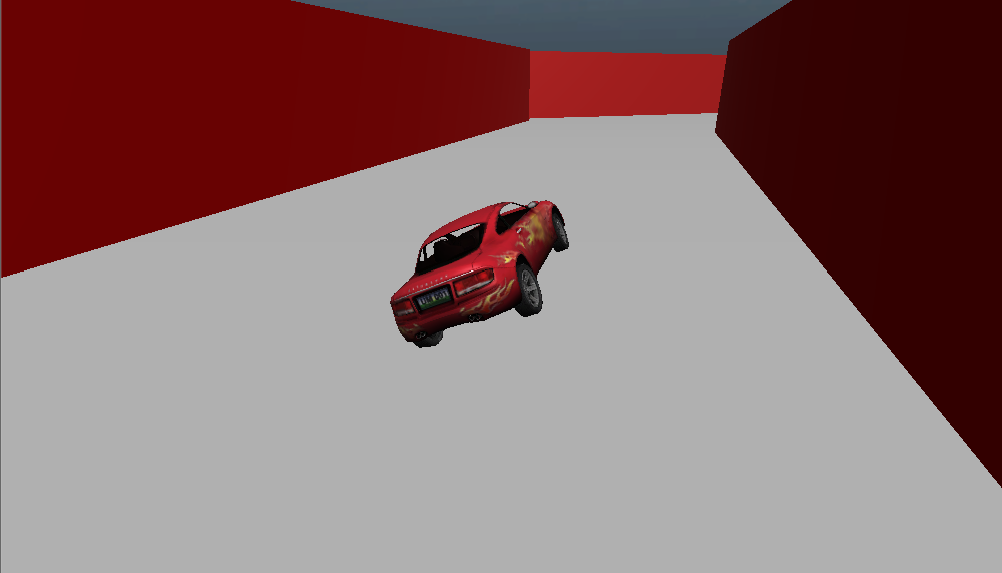
\includegraphics[scale=0.4]{prototype.png}
\end{center}

\section{Bibliography TODO EXPORT TO MAIN}
Agile Way of Working (Scrum Guide) - Bank of America Merrill Lynch

Scrum Principles and Practices
https://www.scrumalliance.org/

Lean Startup (E. Ries)
http://www.amazon.co.uk/The-Lean-Startup-Innovation-Successful/dp/0670921602/

Scaling Lean \& Agile Development (C. Larman and B. Vodde)
http://www.amazon.co.uk/Scaling-Lean-Agile-Development-Organizational/dp/0321480961/
